
% \subsection{Statistical and mesh independence study}
\tb{Should i put the number of realization is abs $\omega$}

In the aim of providing accurate closure terms it is of primary importance to verify the well convergence of the mean quantities, either by varing the mesh definition domain size and duration of simulation.
To tackle this problem we carried out four simulation with 125 rising droplets with different mesh definition. 
The flow parameters for this validation read as,  
\begin{align*}
    \mu_r = 0.1,
    && \rho_r = 1.11,
    && Bo = 1,
    && Ga = 75,
    && \phi = 0.1,
    && N_b =125. 
\end{align*}
Note that in these simulations we used a number of $125$ droplets.  
In \ref{ap:A} we give more details on this choice and show that for our concerns it is a sufficient number of droplets. 

\ref{fig:Re_and_Tc}(left) display the cumulative mean of the vertical Reynolds number based on the drift velocity, namely,
\begin{equation}
    \widetilde{Re}(t)
    = \frac{\rho_f d}{\mu_f t}\int_{t_0}^{t_0+t} \left(\Xavg{\textbf{u}^0_d} -  \Xavg{\textbf{u}_c^0}\right)dt'
\end{equation}
\tb{ time average and volume average}
where $t_0$ is the starting sampling time. 
We remark a significant dependence of $\tilde{Re}$ with the mesh definition in contrast to the latter study (see \ref{fig:ordered_array}). 
It is hard to distinguish the cause of this difference, if it is not just because of the presence of interaction between droplets. 
Anyhow, we reach mesh independent results for $d/\Delta \geq 30$ in agreements with the recent studies of \citet{loisy2017buoyancy} \citet{zhang2021direct} for low inertial bubbly flows.
Also, $\widetilde{Re}$ reaches a constant values from $t^* = 50$. 
This is true for all mesh definition.  
Consequently, we reached an accurate time convergence for the rising velocity. 
\begin{figure}[h!]
    \centering
    % 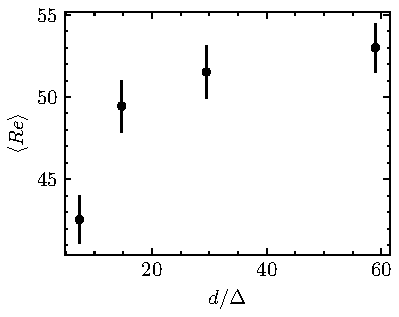
\includegraphics[height = 0.3\textwidth]{image/VALIDATION2.0/fCA/Re.pdf}
    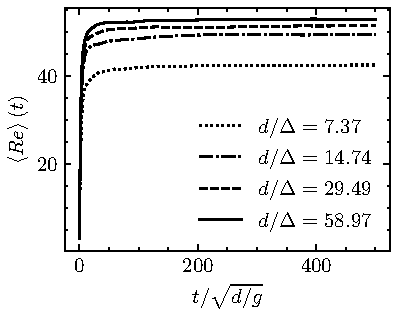
\includegraphics[height = 0.3\textwidth]{image/VALIDATION2.0/fCA/Recum.pdf}
    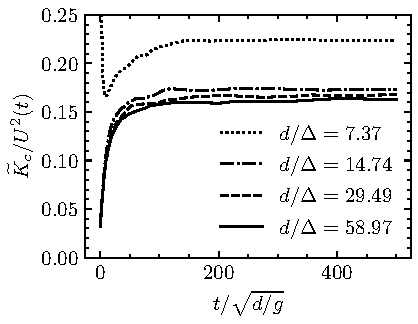
\includegraphics[height = 0.3\textwidth]{image/VALIDATION2.0/fCA/Tcum.pdf}
    % 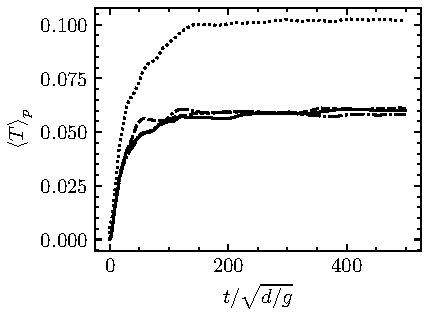
\includegraphics[height = 0.35\textwidth]{image/VALIDATION2.0/fPA/Tcum.pdf}
    \caption{(left) Cumulative mean of the volume averaged Reynolds number along the simulation time based on the drift velocity $U = \textbf{u}_p - \textbf{u}_c$, with $\phi = 0.1$, $\rho_r = 1.11$, $ \mu_r =0.1$ and $Ga = 29.9$ and $N_b = 125$.
    (right) Cumulative mean of the fluid Reynolds stress tesor. }
    \label{fig:Re_and_Tc}
\end{figure}

The well convergence of the rising velocity doesn't guarantee a statistical nor a mesh convergence for finer quantities such as the pseudo-turbulent kinetic energy. 
Therefore, we provide on \ref{fig:UpUp} (left) the running average of the fluid phase pseudo-turbulent energy. 
Similarly, \ref{fig:UpUp} (right) represent the particle center of mass pseudo-turbulent kinetic energy. 
\begin{figure}[h!]
    \centering
    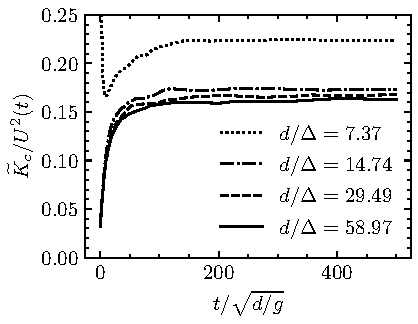
\includegraphics[height = 0.3\textwidth]{image/VALIDATION2.0/fCA/Tcum.pdf}
    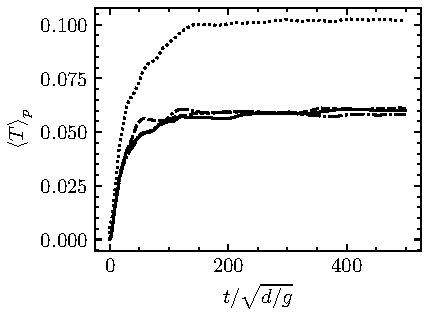
\includegraphics[height = 0.3\textwidth]{image/VALIDATION2.0/fPA/Tcum.pdf}
    \caption{(left) Cumulative mean of the volume averaged granular temperature along the simulation time based on the drift velocity $U = \textbf{u}_p - \textbf{u}_c$, with $\phi = 0.1$, $\rho_r = 1.11$, $ \mu_r =0.1$ and $Ga = 29.9$ and $N_b = 125$.
    (right) Cumulative mean of the dimensionless particle-fluid-particle stress horizontal component tensor. }
    \label{fig:UpUp}
\end{figure}
Both figure exhibit well converged data. 
Interestingly, $\widetilde{K}_c$ and $\widetilde{K}_\alpha$ reach a constant value at $t^* = 200$ which is four time greater than for $\widetilde{Re}$.


\tb{this convergence can be compared to Loisy studies}
\tb{Cite and compare to Berner and \citet{bunner2002dynamics} which found that Nb > 12 is sufficient \citet{roghair2011drag}}
Now, let's investigate the required number of droplets per domain, $N_b$, and the minimum definition of cells per diameter of droplets $\delta$.  
\tb{Include bibliography and expectation here \ldots}
For this investigation we kept the physical parameters presented in the same section and made a double parametric analysis over $N$ and $\delta$. 
We carried out simulations for $N = 2, 3, 4, 5, 6, 7$, and for a number of cells $10 <\delta < 40$. 
In Basilisk the mesh definition is defined by a power of two, consequently depending on the size of the domain (which is fixed to keep a $\phi$ constant) the $\delta$ parameter is fixed at a power of 2 close. 
\begin{figure}[h!]
    \centering
    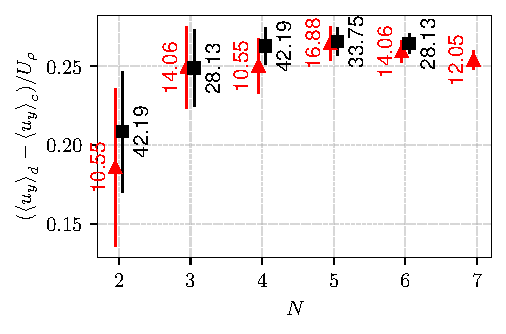
\includegraphics[height= 0.3\textwidth]{image/VALIDATION/N_and_delta/DUd.pdf}
    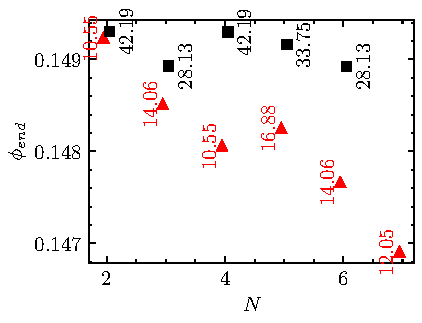
\includegraphics[height= 0.3\textwidth]{image/VALIDATION/N_and_delta/PHI.pdf}
    \caption{(left) Averaged Reynolds number based on the drift velocity.
            (right) Dispersed phase volume fraction at the end of each simulation.
            The text on the side of the points is $\delta$.
            N correspond to $N = N_b^3$. }
    \label{fig:VALIDATION_Nd_1}
\end{figure}
\ref{fig:VALIDATION_Nd_1}(left), illustrate clearly that the drift velocity is independent of the parameters $N_b$ and $\delta$, for $N >4$. 
On the other hand, \ref{fig:VALIDATION_Nd_1}(right), show that the volume fraction of the dispersed phase is lower for the low defined grid (red dots), due to a loss of volume during the simulation.
This doesn't mean that the solver isn't volume conservative. 
In fact, it is fund to be due to the \href{http://basilisk.fr/sandbox/fintzin/Rising-Suspension/no-coalescence.h}{no-coalescence.h} which generate fragment into the numerical domain, fragment which are deleted in the long run. 
\begin{figure}[h!]
    \centering
    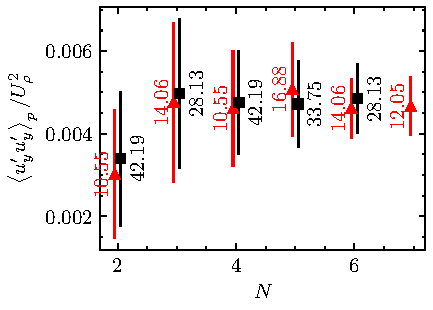
\includegraphics[height= 0.3\textwidth]{image/VALIDATION/N_and_delta/PA_UpUp.pdf}
    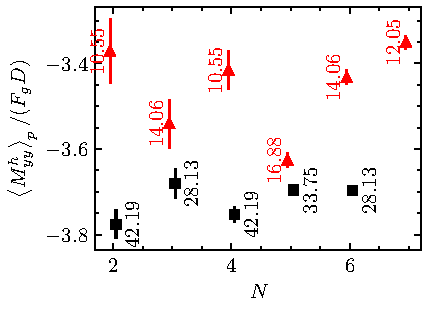
\includegraphics[height= 0.3\textwidth]{image/VALIDATION/N_and_delta/Mh.pdf}
    \caption{(left) Fluids phase averaged fluctuation tensor.
            (right) Particular average of the first moment tensor, where $F_g$ is the buoyancy force applied on one droplet. 
            The numerical values displayed alongside the dots are the number of cells per diameter.}
    \label{fig:VALIDATION_Nd_2}
\end{figure}
Now, let's look at the behavior of more \textit{complicated} closure terms. 
\ref{fig:VALIDATION_Nd_2}(left) demonstrate that the vertical component of the pseudo turbulent tensor is parameter independent rather early, independently of the grid definition. 
This fact is rather surprising but note that the standard deviation is quite high for small domain. 
On \ref{fig:VALIDATION_Nd_2}(right), we can examine the vertical component of the first moment closure term. 
It is found to be constant for all $N$, but rather inaccurate for coarse grids. 
Which makes sens since the first moment results from a local calculation of the stress over a droplet volume, unlike the other quantities which results from the averaged center of mass velocity of a droplet. 

As we have shown, the quantities presented converge for a number of droplets equivalent to $N = 4$ and $\delta = 25$. 
Thus, we validate our simulation in space, i.e. we made sure that our domain were wide enough to minimize the influence of the periodicity on our results, and in mesh definition. 
Nevertheless, at it is the number of realization that matter when carrying a particular average, it is interesting to look at the duration of the simulation.


The last validation that we must expose is the convergence with the relative properties. 
Indeed, the film definition might change interaction properties such that the particle normal approach $\textbf{w}_n(a)$. 
\begin{figure}[h!]
    \centering
    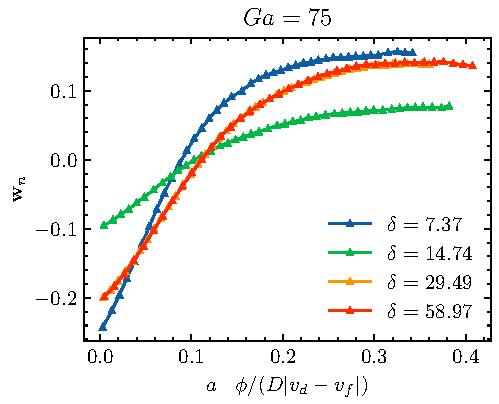
\includegraphics[height=0.3\textwidth]{image/VALIDATION2.0/Hnst/ur_a_ndc_35_Ga_75.pdf}
    \caption{Normal approach Nearest particle velocity for different $Ga$. 
    We can see that for $\delta = 29,60$ we obtain the same results.}
\end{figure}

